\documentclass{beamer}

\mode<presentation> {

\usepackage{beamerthemeAmsterdam}
\usecolortheme{dolphin}
\usepackage{hyperref}

%\setbeamertemplate{footline} % To remove the footer line in all slides uncomment this line
%\setbeamertemplate{footline}[page number] % To replace the footer line in all slides with a simple slide count uncomment this line

%\setbeamertemplate{navigation symbols}{} % To remove the navigation symbols from the bottom of all slides uncomment this line
}

\usepackage{graphicx} % Allows including images
\usepackage{booktabs} % Allows the use of \toprule, \midrule and \bottomrule in tables

%----------------------------------------------------------------------------------------
%	TITLE PAGE
%----------------------------------------------------------------------------------------
\title[Movement of Ants]{Computational Science: Movement of Ants} % The short title appears at the bottom of every slide, the full title is only on the title page

\author{Georgios Methenitis} % Your name
\institute[UVA] % Your institution as it will appear on the bottom of every slide, may be shorthand to save space
{

\includegraphics[width=0.3\textwidth]{UvA-logo-english.jpg}
}
\date{\today} % Date, can be changed to a custom date

\begin{document}

\begin{frame}
\titlepage % Print the title page as the first slide
\end{frame}

\begin{frame}
\frametitle{Overview} % Table of contents slide, comment this block out to remove it
\tableofcontents % Throughout your presentation, if you choose to use \section{} and \subsection{} commands, these will automatically be printed on this slide as an overview of your presentation
\end{frame}

%----------------------------------------------------------------------------------------
%	PRESENTATION SLIDES
%----------------------------------------------------------------------------------------

%------------------------------------------------
\section{Introduction} 
\begin{frame}
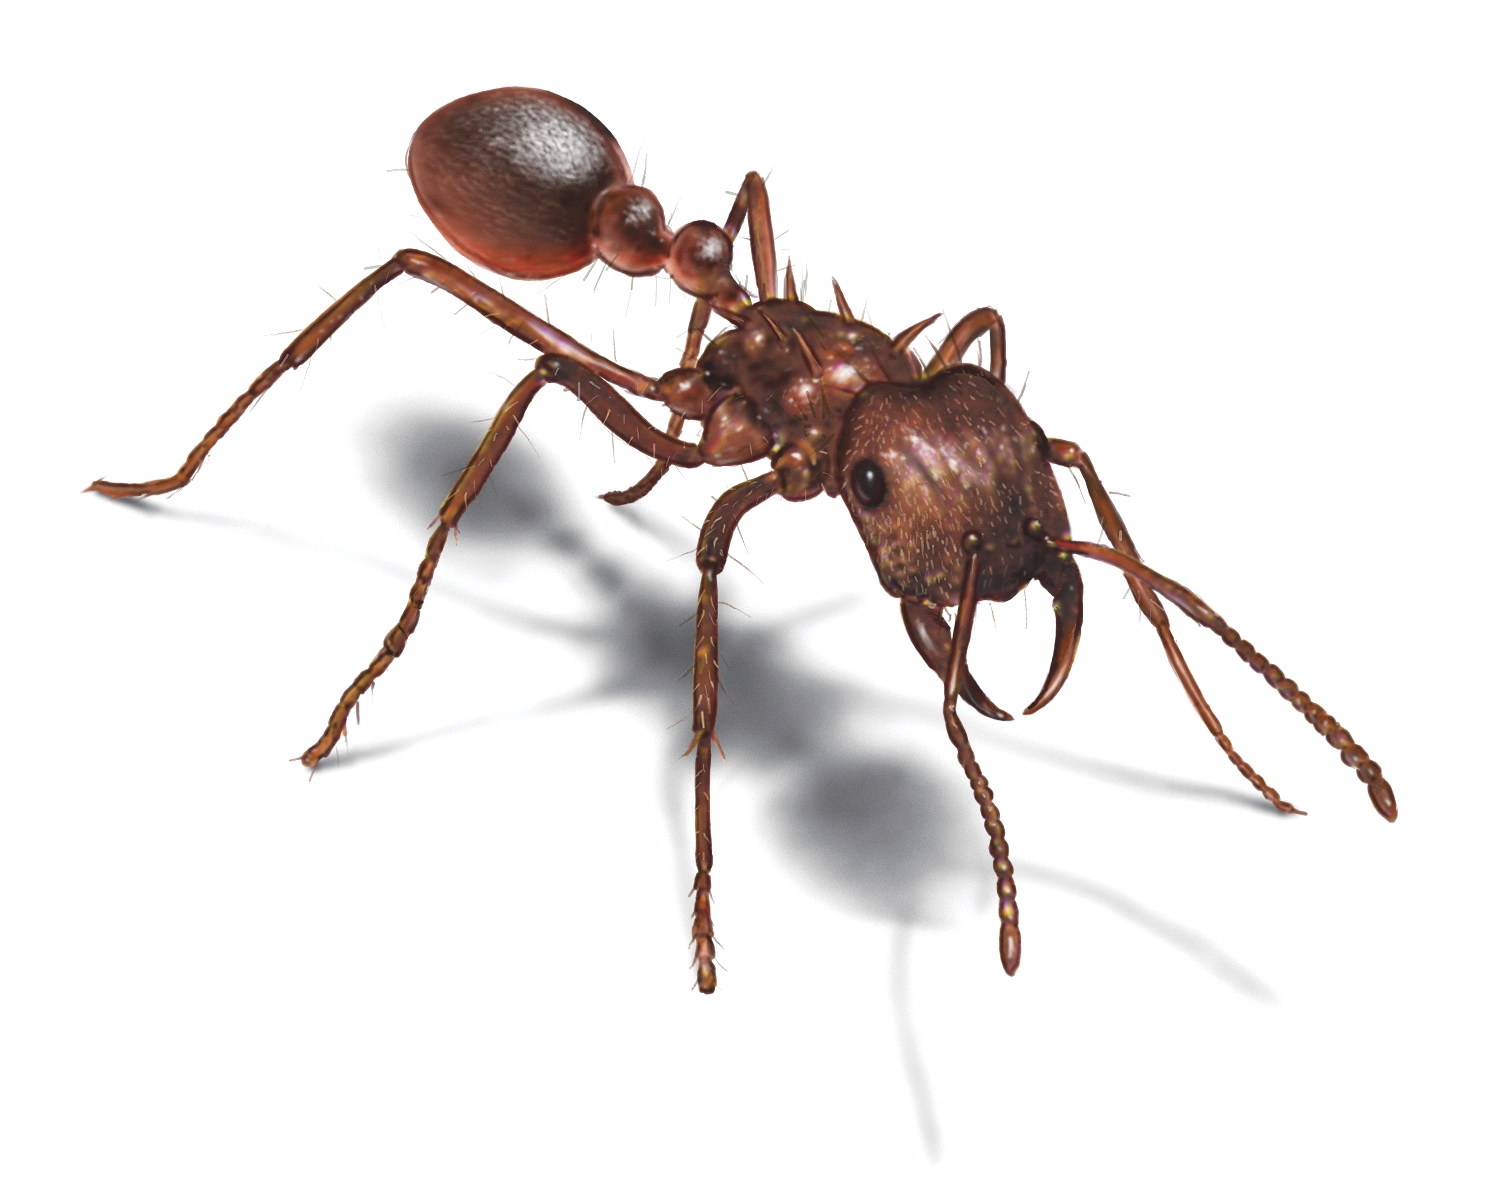
\includegraphics[width=0.3\textwidth]{ant-02.jpg}
\begin{itemize}
\item Ants are social insects of the family Formicidae.
\item Big ants' average speed is 300 meters per hour. (Human 18 m/h).
\item Foraging ants travel distances of up to 200 meters from their nest.
\item Ants communicate with each other using \textbf{pheromones}, sounds, and touch.
\end{itemize}
\end{frame}

\section{Approach}
\begin{frame}
Approach to the problem
\begin{itemize}
\item Grid $2$D space, $500 \times 500 !$
\item Nest, Food, points in $2$D space.
\item Obstacles
\item Two kinds of pheromone
\item Home, food pheromone
\item Ants independent agents
\item Random ant movement only to neighbor cells
\item $\epsilon$-greedy approach
\item Diffusion, evaporation
\end{itemize}
\end{frame}

\begin{frame}[allowframebreaks]
How the simulation works:
\begin{itemize}
\item Initially all ants located at their nest
\item Their hunger level is $h = 1.0$, $h \in [0.0,1.0]$
\item $h = 1.0$, means they are starving
\item They start a random walk
\item They are dropping home pheromone as they are located in their nest:
\begin{equation}
{ph\_{home}}_t^{i,j} = max\_ph\_home, if\ i,j = nest
\end{equation}
\item When they move they take with them the pheromone:
\begin{equation}
{ph\_{home}}_t^{i,j} = \smash{\displaystyle\max_{-1 \leq x,y \leq 1}}[{ph\_{home}}_{t-1}^{i+x,j+y}] - \beta,\ x,y \in \mathbb{R}
\end{equation}
\item instead:
\begin{equation}
{ph\_{home}}_t^{i,j} = {ph\_{home}}_{t-1}^{i,j} - \beta
\end{equation}
\item When food is located in the same cell as an ant is:
\begin{equation}
{ph\_{food}}_t^{i,j} = max\_ph\_food, if\ i,j = food
\end{equation}
\item Ants leave trails as they move out from the food source, with the same way they do for home. But now they are dropping food pheromone.
\item Value Iteration?
\item When the ants have $h < hunger\_threshold$, $0.3$ is used. They want to go back at their nest.
\item When the ants have $h \geq hunger\_threshold$. They want to go find food again.
\end{itemize}
\end{frame}


\begin{frame}
Epsilon-greedy action selection:
\begin{itemize}
\item The best action is selected for a proportion $1 - \epsilon$ of the trials, and another action is randomly selected for a proportion $\epsilon$.
\item A typical parameter that is used is: $\epsilon = 0.2$, but this can vary.
\item Depending where they want to go, they follow with $\epsilon$-greedy the  pheromone.
\item When greedy action is chosen, ants select the cell with the maximum pheromone.
\end{itemize}
\end{frame}

\begin{frame}
Diffusion:
\begin{equation}
{ph}_t^{i,j} = max[{ph}_{t-1}^{i,j}, r_d * \smash{\displaystyle\max_{-1 \leq x,y \leq 1}}[{ph}_{t-1}^{i+x,j+y}], x,y \in \mathbb{R}
\end{equation}
$r_d \in [0.0,1.0]$, diffusion rate.\\
\vspace{0.6cm}
Evaporation:
\begin{equation}
{ph}_t^{i,j} = r_e * {ph}_{t-1}^{i,j}
\end{equation}
$r_e \in [0.0,1.0]$, evaporation rate.\\
\end{frame}

\section{Results}
\begin{frame}
Map:\\
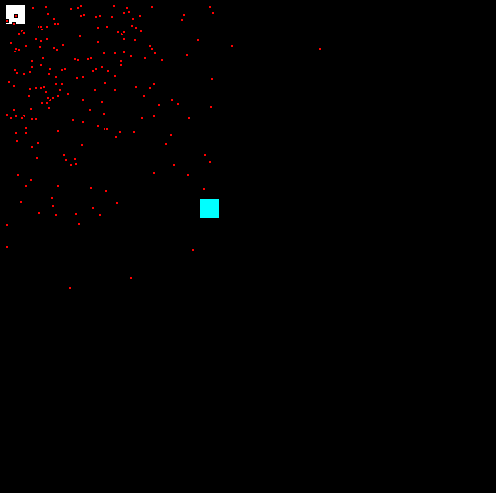
\includegraphics[width=0.7\textwidth]{map.png}
\end{frame}

\begin{frame}
Gui:\\
\vspace{0.3cm}
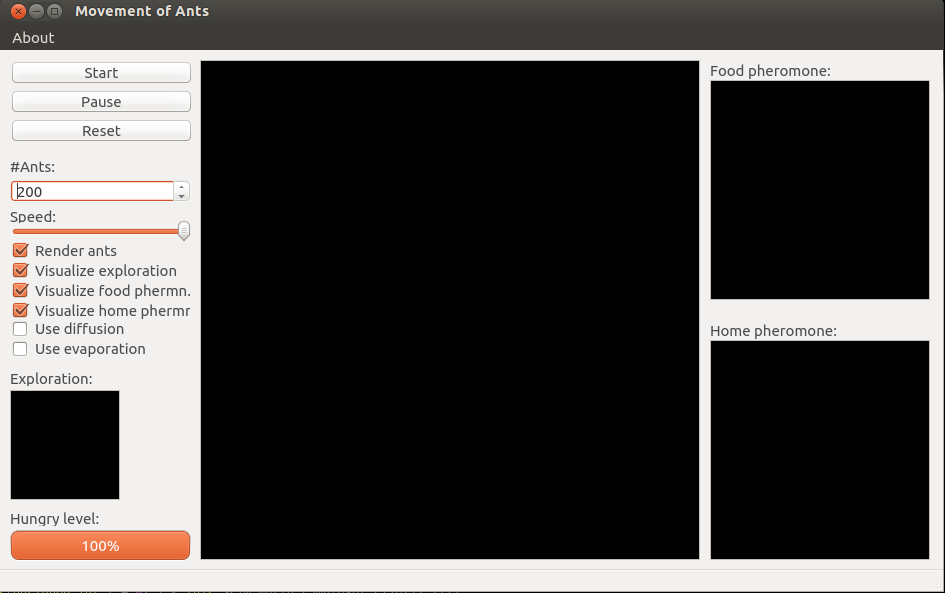
\includegraphics[width=1.0\textwidth]{gui.png}
\end{frame}


\begin{frame}
Experiment(No obstacle)\\
\vspace{0.3cm}
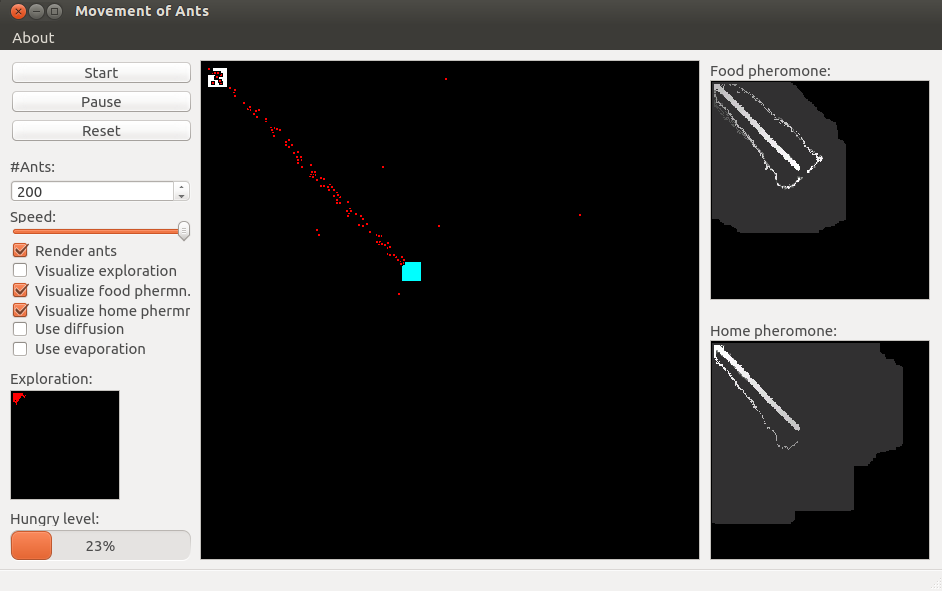
\includegraphics[width=1.0\textwidth]{noObstacle.png}
\end{frame}


\begin{frame}
Experiment(With obstacle)\\
\vspace{0.3cm}
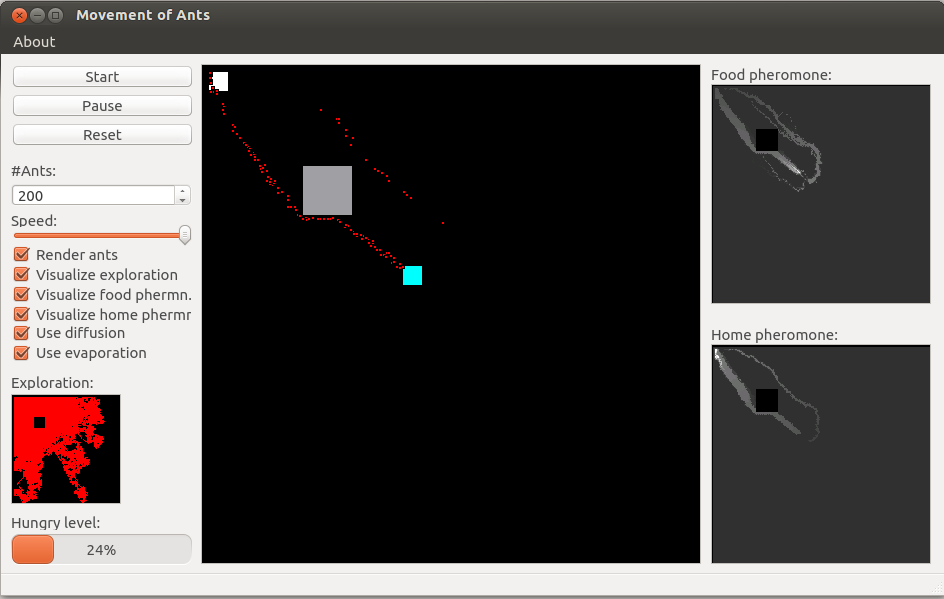
\includegraphics[width=1.0\textwidth]{obstacle.png}
\end{frame}

\section{Demo}
\begin{frame}
\Huge{\centerline{Demo}}
\end{frame}

\section{Future Work}
\begin{frame}
Future Work:
\begin{itemize}
\item Include also death, born rates.
\item Make the simulation more realistic, constants, distances, etc..
\end{itemize}
Source code: 
\begin{itemize}
\item github.com/GiorgosMethe/AntsMovement
\end{itemize}
\end{frame}


\begin{frame}
\frametitle{References}
\footnotesize{
\begin{thebibliography}{99} % Beamer does not support BibTeX so references must be inserted manually as below
\bibitem[Paulo E. Merloti]{p1} Paulo E. Merloti
\newblock Simulation of Artificial Ant’s Behavior 
in a Digital Environment.
\newblock \emph{Department of Computer Science 
Graduate Seminar in Artificial Intelligence 
Evolutionary and Adaptive Computation 
}

\bibitem[Liviu A. Panait and Sean Luke
]{p1} Liviu A. Panait and Sean Luke
\newblock Ant Foraging Revisited
\newblock \emph{George Mason University, Fairfax, VA 22030
lpanait@cs.gmu.edu, sean@cs.gmu.edu
}




\bibitem[Online]{p2}\href{http://www.ehow.com/about_5365350_fast-can-ant-run.html}{How Fast Can an Ant Run?}
\bibitem[Online]{p2}\href{http://en.wikipedia.org/wiki/Ant}{Wiki: Ant}
\bibitem[Online]{p2}\href{http://en.wikipedia.org/wiki/Ant_colony_optimization_algorithms}{Ant colony optimization algorithms}

\end{thebibliography}
}
\end{frame}

%------------------------------------------------

\begin{frame}
\Huge{\centerline{The End}}
\end{frame}

%----------------------------------------------------------------------------------------

\end{document}